\documentclass[a4paper, 11pt]{article}
\usepackage{amsmath}
\usepackage{graphicx}
\usepackage{geometry}
\usepackage{listings}
\geometry{scale=0.8}
\linespread{1.5}
\usepackage{hyperref}
\usepackage{color}
\definecolor{dkgreen}{rgb}{0,0.6,0}
\definecolor{gray}{rgb}{0.5,0.5,0.5}
\definecolor{mauve}{rgb}{0.58,0,0.82}
\lstset{frame=shadowbox,
    language=python,
    aboveskip=3mm,
    belowskip=3mm,
    showstringspaces=false,
    columns=flexible,
    basicstyle={\small\ttfamily},
    keywordstyle=\color{blue},
    commentstyle=\color{dkgreen},
    stringstyle=\color{mauve},
    breaklines=true,
    breakatwhitespace=true,
    tabsize=3,
    numbers=left
}

\usepackage[UTF8, scheme=plain, punct=plain, zihao=false]{ctex}

\title{	
\normalfont \normalsize
\textsc{School of Data and Computer Science, Sun Yat-sen University} \\ [25pt] %textsc small capital letters
\rule{\textwidth}{0.5pt} \\[0.4cm] % Thin top horizontal rule
\huge  E10 Variable Elimination \\ % The assignment title
\rule{\textwidth}{2pt} \\[0.5cm] % Thick bottom horizontal rule
\author{17341203 Yixin Zhang}
\date{\normalsize\today}
}

\begin{document}
\maketitle
\tableofcontents
\newpage


\section{VE}

The burglary example is described as following:
\begin{figure}[h]
  \centering

  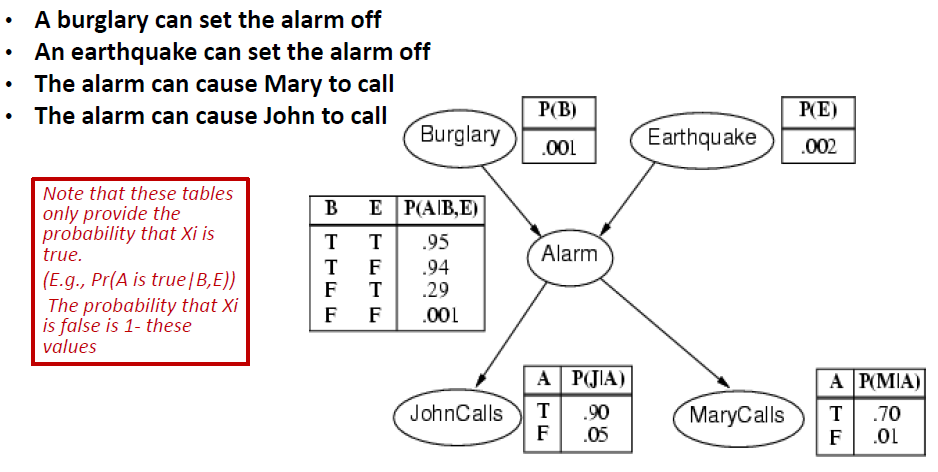
\includegraphics[width=14cm]{Pic/burglary}
\end{figure}

\begin{figure}[ht]
\centering
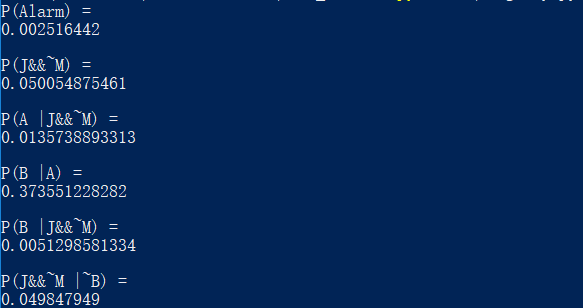
\includegraphics[width=12cm]{Pic/burglar_result}
\end{figure}
Here is a VE template for you to solve the burglary example:
\begin{lstlisting}[language=Python,frame=single]
class VariableElimination:
    @staticmethod
    def inference(factorList, queryVariables, 
    orderedListOfHiddenVariables, evidenceList):
        for ev in evidenceList:
            #Your code here
        for var in orderedListOfHiddenVariables:
            #Your code here
        print "RESULT:"
        res = factorList[0]
        for factor in factorList[1:]:
            res = res.multiply(factor)
        total = sum(res.cpt.values())
        res.cpt = {k: v/total for k, v in res.cpt.items()}
        res.printInf()
    @staticmethod
    def printFactors(factorList):
        for factor in factorList:
            factor.printInf()
class Util:
    @staticmethod
    def to_binary(num, len):
        return format(num, '0' + str(len) + 'b')
class Node:
    def __init__(self, name, var_list):
        self.name = name
        self.varList = var_list
        self.cpt = {}
    def setCpt(self, cpt):
        self.cpt = cpt
    def printInf(self):
        print "Name = " + self.name
        print " vars " + str(self.varList)
        for key in self.cpt:
            print "   key: " + key + " val : " + str(self.cpt[key])
        print ""
    def multiply(self, factor):
        """function that multiplies with another factor"""
        #Your code here
        new_node = Node("f" + str(newList), newList)
        new_node.setCpt(new_cpt)
        return new_node
    def sumout(self, variable):
        """function that sums out a variable given a factor"""
        #Your code here
        new_node = Node("f" + str(new_var_list), new_var_list)
        new_node.setCpt(new_cpt)
        return new_node
    def restrict(self, variable, value):
        """function that restricts a variable to some value 
        in a given factor"""
        #Your code here
        new_node = Node("f" + str(new_var_list), new_var_list)
        new_node.setCpt(new_cpt)
        return new_node
# create nodes for Bayes Net
B = Node("B", ["B"])
E = Node("E", ["E"])
A = Node("A", ["A", "B","E"])
J = Node("J", ["J", "A"])
M = Node("M", ["M", "A"])

# Generate cpt for each node
B.setCpt({'0': 0.999, '1': 0.001})
E.setCpt({'0': 0.998, '1': 0.002})
A.setCpt({'111': 0.95, '011': 0.05, '110':0.94,'010':0.06,
'101':0.29,'001':0.71,'100':0.001,'000':0.999})
J.setCpt({'11': 0.9, '01': 0.1, '10': 0.05, '00': 0.95})
M.setCpt({'11': 0.7, '01': 0.3, '10': 0.01, '00': 0.99})

print "P(A) **********************"
VariableElimination.inference([B,E,A,J,M], ['A'], ['B', 'E', 'J','M'], {})

print "P(B | J~M) **********************"
VariableElimination.inference([B,E,A,J,M], ['B'], ['E','A'], {'J':1,'M':0})
\end{lstlisting}
\section{Task}
\begin{itemize}
\item You should implement 4 functions: \texttt{inference}, \texttt{multiply}, \texttt{sumout} and \texttt{restrict}. You can turn to Figure \ref{Fig:ve_product} and Figure \ref{Fig:sumout_restrict} for help. 
\item Please hand in a file named \textsf{E09\_YourNumber.pdf}, and send it to \textsf{ai\_201901@foxmail.com}
\end{itemize}


\begin{figure}[ht]{}
\centering
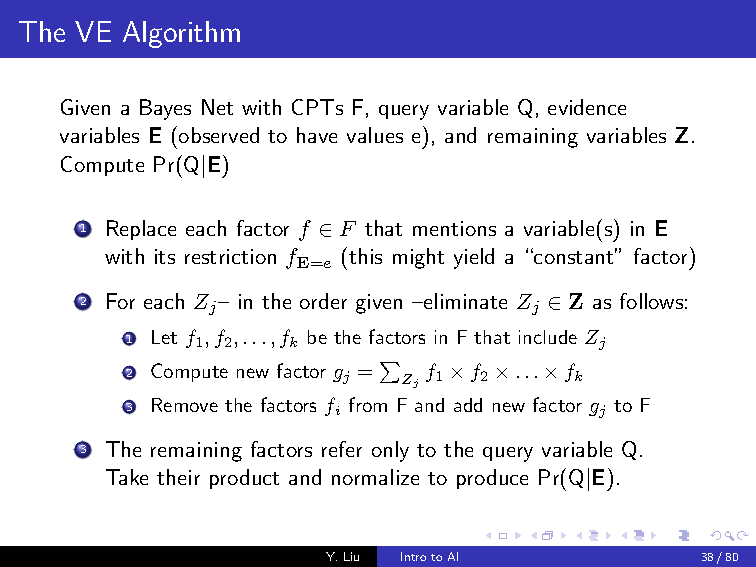
\includegraphics[width=7.5cm]{Pic/ve}
\qquad
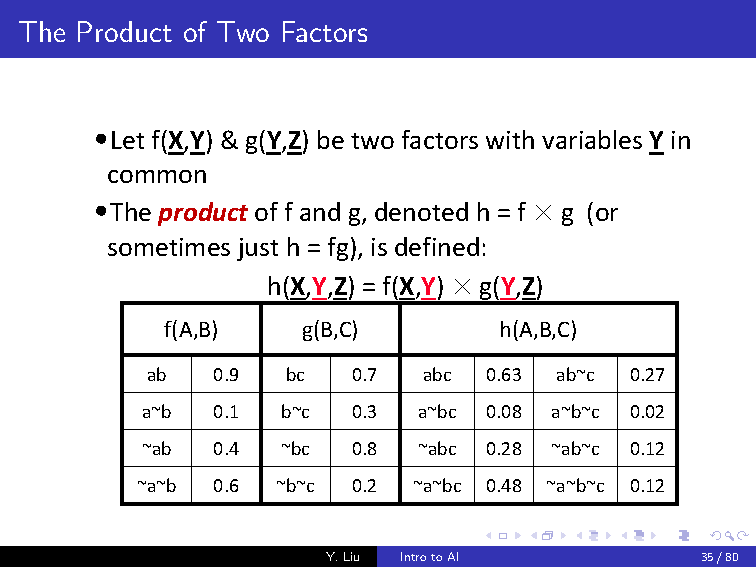
\includegraphics[width=7.5cm]{Pic/product}
\caption{VE and Product}
\label{Fig:ve_product}
\end{figure}


\begin{figure}[ht]
\centering
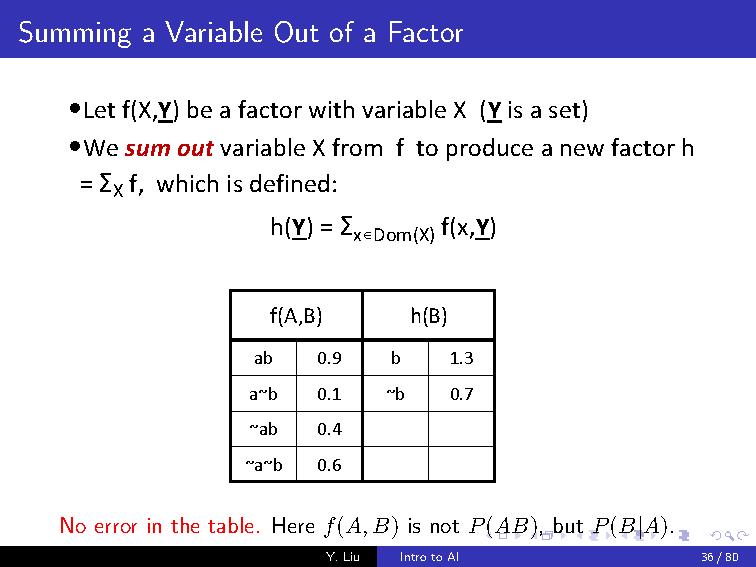
\includegraphics[width=7.5cm]{Pic/sumout}
\qquad
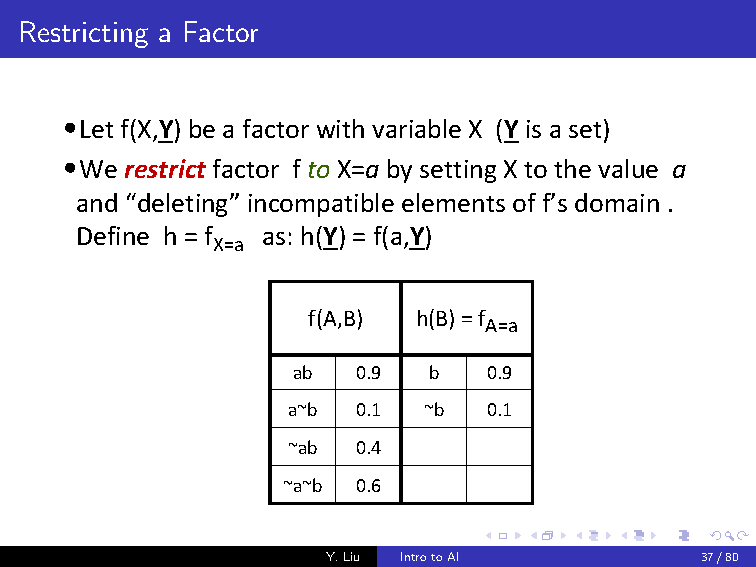
\includegraphics[width=7.5cm]{Pic/restrict}
\caption{Sumout and Restrict}
\label{Fig:sumout_restrict}
\end{figure}



\section{Codes and Results}
\subsection{Overview}
The most difficult part in the code is the implementation of `multiply' method. There, the behaviour of `multiply' is quite similar to that of natural join in relational databases.

Moreover, there are some special cases that must be taken care of in `multiply'. For example, when two factors which are to multiply have no common variables, or one of the factors' variable list is empty, `multiply' method must work correctly.


\subsection{Code}
\begin{lstlisting}
# -*- coding: utf-8 -*-
# @Author: Jed Zhang 
# @Date: 2019-11-16 10:49:40

class VariableElimination:
    @staticmethod
    def inference(factorList, queryVariables, orderedListOfHiddenVariables, evidenceList):
        # Step 1: 用证据取代factor中相关变量的值
        for ev in evidenceList:
            for i, factor in enumerate(factorList):
                if ev in factor.varList:  # 因子中有变量在证据中
                    factorList[i] = factor.restrict(ev, evidenceList[ev])
            
        # Step 2: 按顺序依次消除变量
        for var in orderedListOfHiddenVariables:  # var就是课件里的Zj
            corresponding_factors = [factor for factor in factorList if var in factor.varList]
            if corresponding_factors:
                new_factor = corresponding_factors[0]
                factorList.remove(new_factor)
                for factor in corresponding_factors[1:]:  # 从第二个开始累乘
                    new_factor = new_factor.multiply(factor)
                    factorList.remove(factor)
                new_factor = new_factor.sumout(var)  # 对变量求和从而消除该变量
            factorList.append(new_factor)

        # Step 3: 归一化并显示结果
        print("RESULT:")
        res = factorList[0]
        for factor in factorList[1:]:
            res = res.multiply(factor)
        total = sum(res.cpt.values())  # 归一化分母
        res.cpt = {k: v/total for k, v in res.cpt.items()}
        res.printInf()

    @staticmethod
    def printFactors(factorList):
        for factor in factorList:
            factor.printInf()


# 并没有用到Util类
# class Util:
#     @staticmethod
#     def to_binary(num, len):
#         return format(num, '0' + str(len) + 'b')


class Node:
    def __init__(self, name, var_list):
        self.name = name
        self.varList = var_list
        self.cpt = {}  # 由setCpt函数输入

    def setCpt(self, cpt):
        self.cpt = cpt

    def printInf(self):
        print("Name = " + self.name)
        print(" vars " + str(self.varList))
        for key in self.cpt:
            print("   key: " + key + " val : " + str(self.cpt[key]))
        print("")

    def multiply(self, factor):
        """function that multiplies with another factor"""
        # 使用了类似关系型数据库中“自然连接”的操作
        var_intersection = sorted(list(set(self.varList) & set(factor.varList)))  # 两个factor的变量交集
        new_var_list = self.varList + [var for var in factor.varList if var not in var_intersection]
        tup_index1 = [self.varList.index(x) for x in var_intersection]
        tup_index2 = [factor.varList.index(x) for x in var_intersection]
        
        merge_tup = list(zip(tup_index1, tup_index2))
        new_cpt = {}
        for key1 in self.cpt:
            for key2 in factor.cpt:
                flag = True
                for m in merge_tup:
                    if key1[m[0]] != key2[m[1]]:  # 不符合自然连接条件,跳过当前key对
                        flag = False
                        break
                if flag:
                    # key1+temp组成新的key
                    temp = key2
                    for m in merge_tup:
                        temp = list(key2)
                        temp[m[1]] = 'x'  # 用x标记该字符将要删除
                        temp = ''.join(temp).replace('x', '')
                    new_cpt[key1+temp] = self.cpt[key1] * factor.cpt[key2]

        new_node = Node("f" + str(new_var_list), new_var_list)
        new_node.setCpt(new_cpt)
        return new_node

    def sumout(self, variable):
        """function that sums out a variable given a factor"""
        pos = self.varList.index(variable)  # 要求和的变量的序号
        new_var_list = self.varList[:pos] + self.varList[pos+1:]

        new_cpt_keyset = sorted(list(set([k[:pos]+k[pos+1:] for k in self.cpt.keys()])))  # 新变量列表的组合构成的集合
        new_cpt = {}
        for new_key in new_cpt_keyset:
            new_value = 0
            for value in ['0', '1']:  # 本例中变量只有两种取值
                new_value += self.cpt[new_key[:pos] + value + new_key[pos:]]  # 在原来的CPT中进行累加
            new_cpt[new_key] = new_value

        new_node = Node("f" + str(new_var_list), new_var_list)
        new_node.setCpt(new_cpt)
        return new_node
        
    def restrict(self, variable, value):
        """function that restricts a variable to some value in a given factor"""
        pos = self.varList.index(variable)  # 要限制的变量的序号
        new_var_list = self.varList[:pos] + self.varList[pos+1:]

        new_cpt_keyset = sorted(list(set([k[:pos]+k[pos+1:] for k in self.cpt.keys()])))  # 新变量列表的组合构成的集合
        new_cpt = {}
        for new_key in new_cpt_keyset:
            new_cpt[new_key] = self.cpt[new_key[:pos] + value + new_key[pos:]]

        new_node = Node("f" + str(new_var_list), new_var_list)
        new_node.setCpt(new_cpt)
        return new_node


if __name__ == '__main__':
    # create nodes for Bayes Net
    B = Node("B", ["B"])
    E = Node("E", ["E"])
    A = Node("A", ["A", "B","E"])
    J = Node("J", ["J", "A"])
    M = Node("M", ["M", "A"])

    # Generate cpt for each node
    B.setCpt({'0': 0.999, '1': 0.001})
    E.setCpt({'0': 0.998, '1': 0.002})
    A.setCpt({'111': 0.95, '011': 0.05, '110':0.94,'010':0.06,
    '101':0.29,'001':0.71,'100':0.001,'000':0.999})
    J.setCpt({'11': 0.9, '01': 0.1, '10': 0.05, '00': 0.95})
    M.setCpt({'11': 0.7, '01': 0.3, '10': 0.01, '00': 0.99})

    # 注意:下面evidenceList中将变量的取值统一成字符串的'1'的'0',而不是数字。
    print("P(A)", end=' ')
    VariableElimination.inference([B,E,A,J,M], ['A'], ['B', 'E', 'J','M'], {})

    print("P(J&&~M)", end=' ')
    VariableElimination.inference([B,E,A,J,M], ['J', '~M'], ['B', 'E', 'A'], {})

    print("P(A|J&&~M)", end=' ')
    VariableElimination.inference([B,E,A,J,M], ['A'], ['E', 'B'], {'J': '1', 'M': '0'})

    print("P(B|A)", end=' ')
    VariableElimination.inference([B,E,A,J,M], ['B'], ['E', 'J', 'M'], {'A': '1'})

    print("P(B|J&&~M)", end=' ')
    VariableElimination.inference([B,E,A,J,M], ['B'], ['E', 'A'], {'J': '1', 'M': '0'})

    print("P(J&&~M|~B)", end=' ')
    VariableElimination.inference([B,E,A,J,M], ['J', '~M'], ['E', 'A'], {'B': '0'})
\end{lstlisting}

\subsection{Results}
\begin{figure}[ht]
\centering
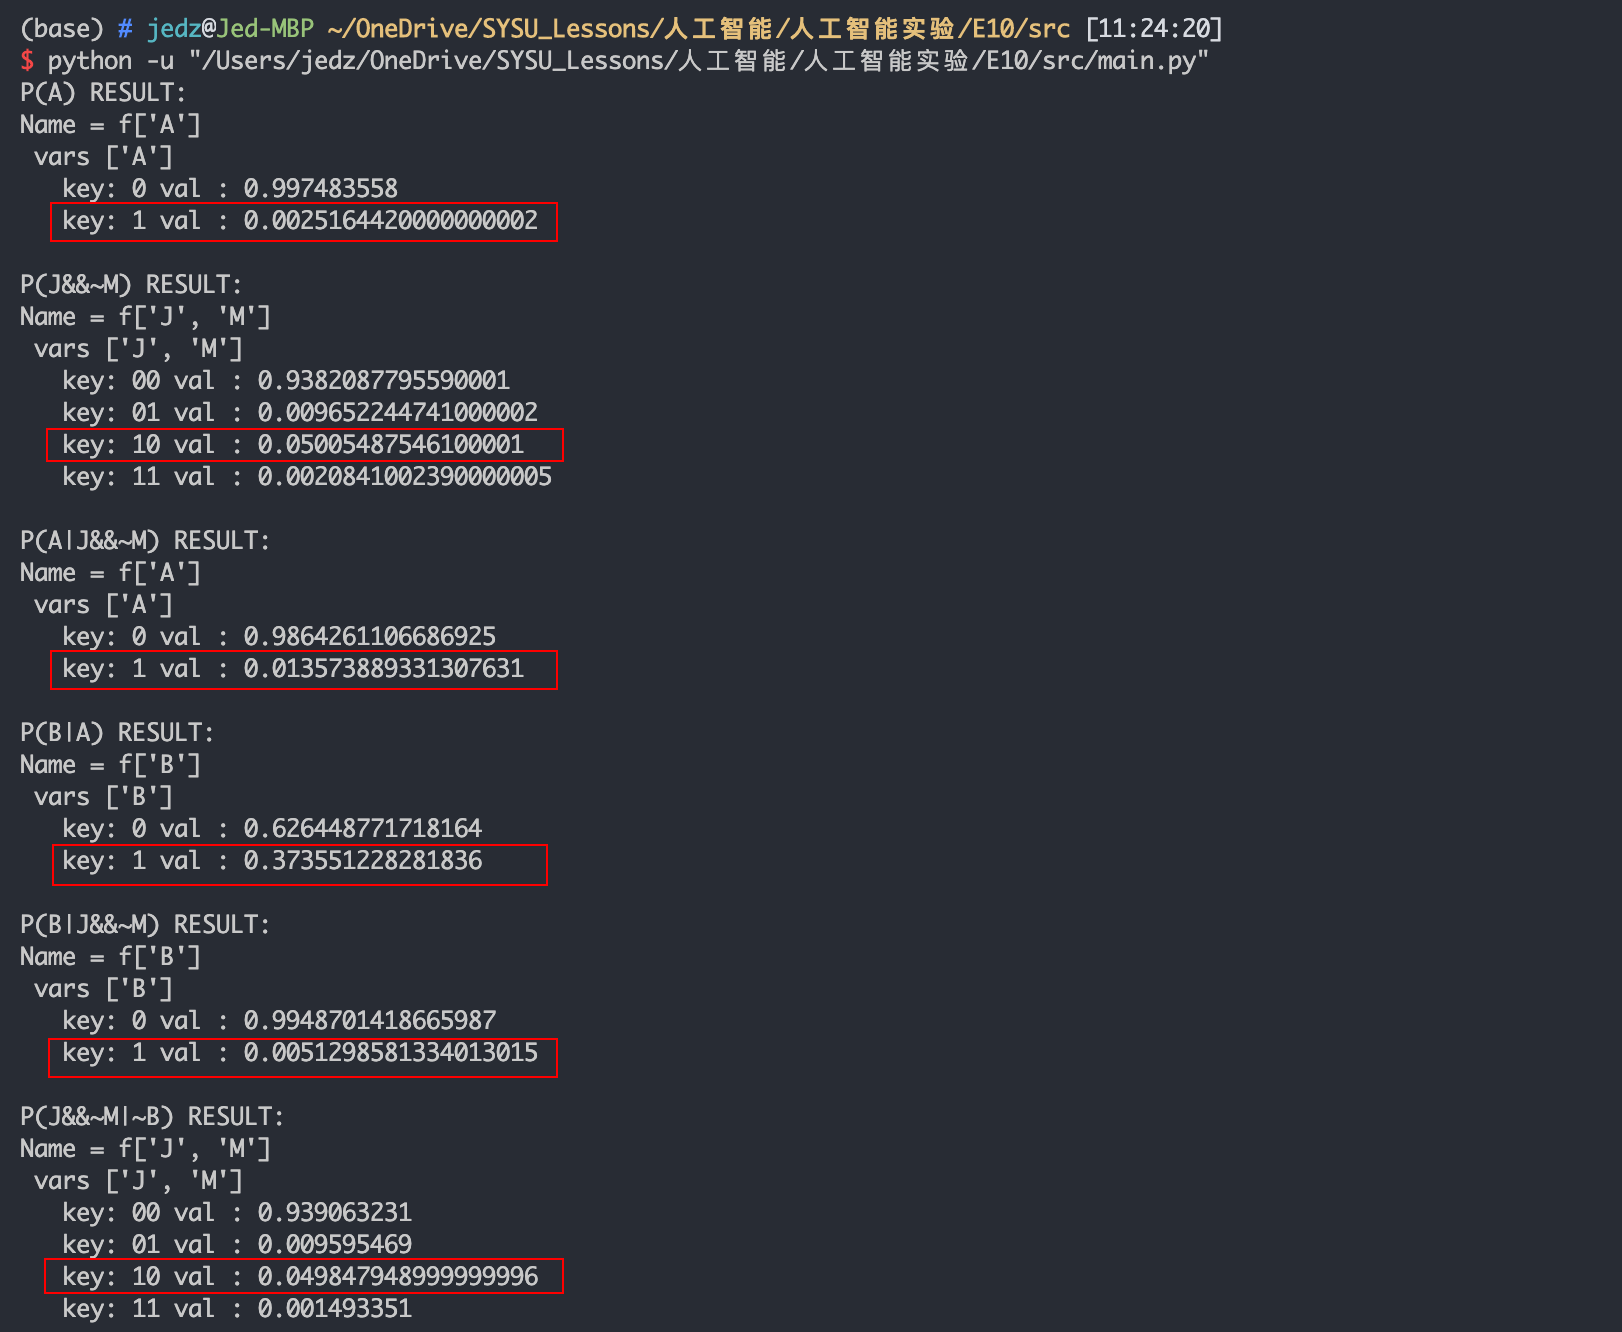
\includegraphics[width=15cm]{Pic/myresults.png}
\end{figure}

%\clearpage
%\bibliography{E:/Papers/LiuLab}
%\bibliographystyle{apalike}
\end{document} 
%%% Local Variables:
%%% mode: latex
%%% TeX-master: t
%%% End:
